\documentclass[11pt,letterpaper]{article}
\usepackage[margin=0.72in]{geometry}
\usepackage{amsmath,amssymb,graphicx,booktabs}
\usepackage[T1]{fontenc}
\usepackage{lmodern}
\usepackage[hidelinks]{hyperref}
\setlength{\parindent}{0pt}
\setlength{\parskip}{4pt}
\setlength{\abovedisplayskip}{6pt}
\setlength{\belowdisplayskip}{6pt}
\setlength{\abovedisplayshortskip}{4pt}
\setlength{\belowdisplayshortskip}{4pt}
\newcommand{\sech}{\operatorname{sech}}
\newcommand{\CleanCoefficient}{2.361111075}
\newcommand{\NoisyCoefficient}{2.361632516}
\newcommand{\CleanP}{1.888888707}
\newcommand{\CleanQ}{0.653594619}
\newcommand{\NoisyP}{1.890135095}
\newcommand{\NoisyQ}{0.654414874}

\hypersetup{pdftitle={From samples to an equation: a magnetic-like kernel benchmark},
pdfauthor={J. R. Landers},
pdfsubject={A controlled verification of kernel regression, equation discovery, integral reconstruction, and recovery of the original analytic function family}}
\begin{document}
\begin{center}
{\Large\bfseries From samples to an equation}\\[3pt]
{\large A magnetic-like kernel benchmark}\\[3pt]
{\small J. R. Landers\quad$\cdot$\quad November 2026}
\end{center}
\vspace{-6pt}

\textbf{Starting question.}
Can a learner that sees only sampled values recover a simple differential relationship,
then solve it to recover the original analytic function family?
We first answer this on a known synthetic example, where a hidden analytic function
provides an independent scoring target. The purpose is to verify the numerical workflow
before interpreting a similar procedure on physical measurements.

\textbf{1. A hidden field and source.}
Let $x$ denote position, $B_*(x)$ a magnetic-like field component, and $J_*(x)$ a
current-like source. All coordinates and channel values are dimensionless. Choose
\begin{equation}
B_*(x)=B_0\tanh(x/L),\qquad J_*(x)=J_0\sech^2(x/L),
\qquad B_*'=a_*J_*,\quad a_*=\frac{B_0}{LJ_0}.
\label{eq:truth}
\end{equation}
Here $B_0=1.7$, $L=0.9$, $J_0=0.8$, and $a_*=85/36$.
For a static geometry $\mathbf B=(0,B(x),0)$ and $\mathbf J=(0,0,J(x))$,
the SI magnetic curl equation reduces to $B'=\mu_0J$; Eq.~\eqref{eq:truth}
is a normalized analogue, not a measurement of permeability.
The learner receives only $b_i=B_*(x_i)+\epsilon_i$ and
$j_i=J_*(x_i)+\eta_i$. Neither the formulas, their constants, nor the true derivatives
are supplied to fitting or model selection.

\textbf{2. Samples become a differentiable representation.}
Fit both channels using the same Gaussian similarity kernel:
\begin{align}
k_\ell(x,x_i)&=e^{-(x-x_i)^2/(2\ell^2)},\qquad
\widehat B(x)=\bar B+\sum_i\alpha_i k_\ell(x,x_i),\quad
\widehat J(x)=\bar J+\sum_i\beta_i k_\ell(x,x_i),\label{eq:fit}\\
[\boldsymbol\alpha\ \boldsymbol\beta]
&=(K+\lambda I)^{-1}(Y-\mathbf1\bar Y),\qquad
\widehat B'(x)=-\sum_i\alpha_i\frac{x-x_i}{\ell^2}k_\ell(x,x_i).
\label{eq:derivative}
\end{align}
$Y$ contains sampled channel values, $K_{ij}=k_\ell(x_i,x_j)$, and the bars are
training means. Validation selects the smoothing length $\ell$ and ridge penalty
$\lambda$ using value predictions. The derivative in Eq.~\eqref{eq:derivative}
is exact for the fitted function; its accuracy for the hidden field is tested separately.

\textbf{3. A representation becomes an equation.}
Search one-, two-, and three-term expressions for $\widehat B'$ from
$\{1,B,J,x,xB,xJ,B^2,BJ,J^2\}$. At fitting positions $z_m$, use learned field values
and separately sampled source values. Select the smallest support meeting a
predeclared 1\% relative derivative-residual tolerance on separate validation positions;
break ties by residual. Both runs select the single term $J$, after which
\begin{equation}
\widehat a=\underset{a}{\arg\min}\sum_m
\bigl[\widehat B'(z_m)-a j_m\bigr]^2,
\qquad \widehat B'\approx\widehat a J.
\label{eq:law}
\end{equation}
The kernel family, coordinate derivative, library, and selection rule are supplied
assumptions. The selected term and its coefficient are learned.

\textbf{4. The equation becomes an integral kernel.}
With one observed boundary value $b_0$ at $x_0=-3$, set
$\kappa_\ell(x,x_i;x_0)=\int_{x_0}^{x}k_\ell(u,x_i)\,du$. Explicitly,
\begin{align}
\kappa_\ell(x,x_i;x_0)&=\ell\sqrt{\frac\pi2}\left[
\operatorname{erf}\!\left(\frac{x-x_i}{\sqrt2\ell}\right)
-\operatorname{erf}\!\left(\frac{x_0-x_i}{\sqrt2\ell}\right)\right],\nonumber\\[-3pt]
\widetilde B(x)&=b_0+\widehat a\!\left[\bar J(x-x_0)
+\sum_i\beta_i\kappa_\ell(x,x_i;x_0)\right],\qquad
\widetilde B'=\widehat a\widehat J.
\label{eq:integral}
\end{align}
The final identity is exact. Agreement of $\widetilde B$ with $B_*$ is a separate
numerical result: the independently fitted $\widehat B$ and integrated $\widetilde B$
need not coincide.

\newpage
\textbf{5. Controlled experiment.}
For each run, draw 80 training positions and 60 kernel-validation positions in
$[-3,3]$. Fit and validate the equation using two further sets of 100 source samples
in $[-2.8,2.8]$, reducing boundary derivative effects. Fix the seed to 20261116.
Select smoothing parameters by channel-standardized validation error.
The second run adds independent Gaussian
noise with standard deviations $0.001B_0$ and $0.001J_0$, including field noise on
the boundary value. These scales are fixed, not relative to each local value.

Only after kernel and equation selection do we reveal the analytic truth and score
901 unseen positions across $[-3,3]$. Equation~\eqref{eq:integral} uses the learned
source and the single boundary reading; no true field curve enters that prediction.

\begin{center}
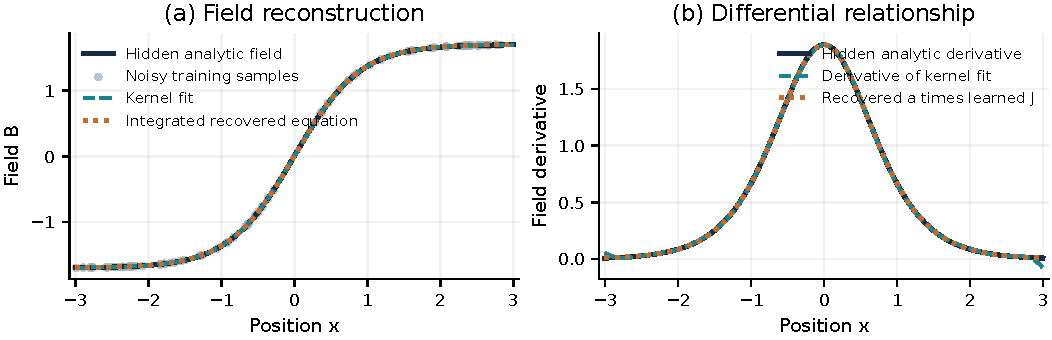
\includegraphics[width=\linewidth]{reconstruction.pdf}
\end{center}
\vspace{-9pt}
{\small\textbf{Figure 1.} The noisy run. (a) Analytic field, sampled values, kernel fit,
and integrated equation agree closely within the sampled interval.
(b) Differentiating the field fit exposes larger errors near the interval boundaries;
the dotted curve uses the recovered coefficient and the learned source.
All axes use normalized units.}

\vspace{4pt}
\textbf{6. Numerical and theoretical results.}
Both runs recover $B'=aJ$ as the simplest accepted expression. The fitted coefficients
are $\widehat a=\CleanCoefficient$ (noiseless) and
$\widehat a=\NoisyCoefficient$ (noisy), versus $a_*=2.361111111\ldots$.
For functions, the table reports $100\|\widehat f-f_*\|_2/\|f_*\|_2$ on the test grid;
for the coefficient it reports $100|\widehat a/a_*-1|$.
\begin{center}
\begin{tabular}{@{}lrr@{}}
\toprule
Relative error (\%) & Noiseless & Noisy \\
\midrule
Field $\widehat B$ & 0.001176 & 0.08535 \\
Derivative $\widehat B'$ & 0.04387 & 1.207 \\
Recovered coefficient $\widehat a$ & $1.52\times10^{-6}$ & 0.02208 \\
Integrated field $\widetilde B$ & $1.26\times10^{-5}$ & 0.2289 \\
\bottomrule
\end{tabular}

\end{center}
\vspace{-4pt}
The theoretical result is Eq.~\eqref{eq:integral}: an exact integral representation
of the selected law for the learned source. Recovery of the original field is
approximate, as quantified above.

\textbf{7. Recovering a function requires another step.}
The Gaussian sum and its integrated error functions do not identify the original
$\tanh/\sech^2$ form. We therefore run a second search, now for an autonomous,
field-only equation: exclude $J$ and $x$, and use $\{1,B,B^2,B^3,B^4\}$.
Use the same fitting/validation positions, maximum of three terms, and 1\% tolerance.
Both runs select the constant and quadratic terms:
\begin{equation}
B'=p-qB^2,\qquad p>0,\quad q>0.
\label{eq:autonomous}
\end{equation}
There are no $\tanh$ or $\sech$ regression features. The restriction to a low-degree
autonomous polynomial equation is a supplied search class; the support and
coefficients come from the kernel reconstruction. All selections, including the
branch and reference value below, finish before scoring against the oracle.

\newpage
\textbf{8. From the learned equation to the original function family.}
Set $A=\sqrt{p/q}$ and $L=1/\sqrt{pq}$. Separating variables in
Eq.~\eqref{eq:autonomous}, on the branch $|B|<A$, gives
\begin{equation}
\int\frac{dB}{p-qB^2}
=\frac{1}{\sqrt{pq}}\operatorname{artanh}(B/A)=x-x_c.
\end{equation}
Inverting and using the previously fitted channel relation $B'=\widehat a J$
recovers the analytic family:
\begin{equation}
\boxed{\ B_{\rm sym}(x)=A\tanh\!\left(\frac{x-x_c}{L}\right),\qquad
J_{\rm sym}(x)=\frac{p}{\widehat a}\sech^2\!\left(\frac{x-x_c}{L}\right).\ }
\label{eq:symbolic}
\end{equation}
Choose $x_r$ as the median training position and $b_r=\widehat B(x_r)$.
Both runs have $|b_r|<A$, selecting the bounded branch and fixing
$x_c=x_r-L\operatorname{artanh}(b_r/A)$. This uses no oracle center and is distinct
from the noisy boundary reading in Eq.~\eqref{eq:integral}.

Analytic integration is supplied mathematics; the data determine the accepted
equation, signs, scales, center and source amplitude. The implementation reports
failure if the selected equation or reference does not support this bounded branch.

\textbf{9. Symbolic recovery results.}
The noisy fit yields $p=\NoisyP$, $q=\NoisyQ$, versus
$p_*=1.888888889\ldots$, $q_*=0.653594771\ldots$. Oracle-scored results follow:
\begin{center}
\small
\begin{tabular}{@{}lrrr@{}}
\toprule
Solved quantity & Noiseless & Noisy & Truth \\
\midrule
Field amplitude $A$ & 1.7 & 1.699495 & 1.7 \\
Transition width $L$ & 0.9000001 & 0.8991393 & 0.9 \\
Center $x_c$ & $4.65\times10^{-8}$ & -0.0006439232 & 0 \\
Source amplitude $p/\widehat a$ & 0.7999999 & 0.8003511 & 0.8 \\
Field error (\%) & $5.67\times10^{-6}$ & 0.04462 & -- \\
Source error (\%) & $1.15\times10^{-5}$ & 0.08857 & -- \\
Derivative error (\%) & $1.16\times10^{-5}$ & 0.09033 & -- \\
Extrapolated field error (\%) & $6.73\times10^{-6}$ & 0.02891 & -- \\
\bottomrule
\end{tabular}

\end{center}
\vspace{-5pt}
\begin{center}
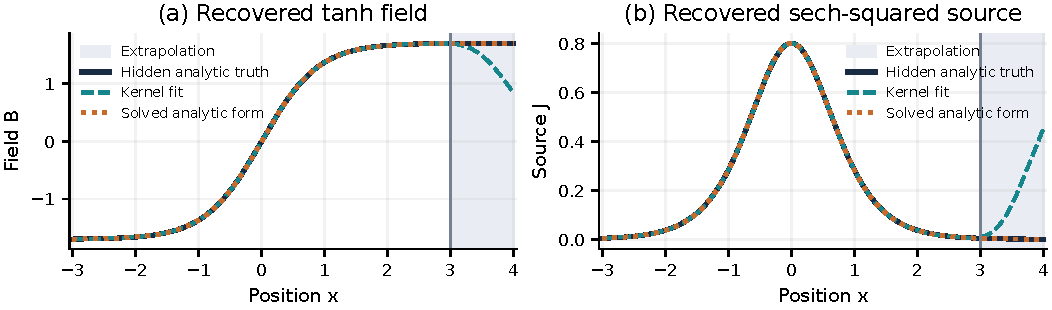
\includegraphics[width=\linewidth]{symbolic_recovery.pdf}
\end{center}
\vspace{-9pt}
{\small\textbf{Figure 2.} The noisy run, now with the solved analytic functions.
Shading marks extrapolation beyond the sampled interval. The original Gaussian
fits depart from the truth there; the recovered $\tanh$ and $\sech^2$ forms remain
close. The two panels use the same learned parameters.}

\vspace{4pt}
\textbf{10. What is now established.}
The original function family is recovered. Its fitted expressions satisfy
$B_{\rm sym}'=p-qB_{\rm sym}^2=\widehat aJ_{\rm sym}$ exactly; agreement with hidden
truth is numerical. Noisy field extrapolation error at $x\in[3.05,4]$ falls from
24\% for the kernel to 0.029\% for the solved equation.

This checks one synthetic family and seed. Polynomial autonomy, smooth kernels,
sparsity and the solution rule are assumptions, not evidence for Maxwell or a unique
physical explanation. The completed chain is \emph{samples $\to$ kernel $\to$
differential equation $\to$ analytic function $\to$ independent scoring positions}.

\vfill
{\footnotesize\raggedright\textbf{Reproducibility.}
From repository root: \texttt{python experiments/kernel\_benchmark/run\_demo.py}.\\
Build all papers: \texttt{python scripts/build\_papers.py}.
Protocol and results: \texttt{experiments/kernel\_benchmark/}.\par}
\end{document}
